\section{ PlanesAndroid }

\subsection { Navigation }

The Android App is built around the so-called Drawer Navigation. This kind of navigation is based on a so-called Hamburger button which in case of the Planes App is displayed in the top left corner of the screen. Tapping on the button displays a list possible destinations in the application. These depend on whether the app is played in the Single Player or Multiplayer Mode. 

In the case of the Single Player App we have:
\begin{itemize}
\item Game
\item Videos
\item Settings
\item Info
\end{itemize}

For the Multiplayer App more screens are available:

\begin{itemize}
	\item Game
	\item Connect to Game
	\item Game Statistics
	\item Login
	\item Logout
	\item Register
	\item Delete User
	\item Videos
	\item Settings
	\item Info
\end{itemize}

When a screen is selected, a Fragment of the Fragment Class corresponding to the screen is loaded into the main layout of the application. The XML layout of the application is shown in \ref{drawer_layout}.

To exemplify how a new screen is loaded onto the screen I show the following function ( \ref{start_norobot_fragment}).

\begin{lstlisting} [caption = {Switch Screen Example},label=start_norobot_fragment]
	fun startNoRobotFragment(regResp : RegistrationResponse) {
		
		mSelectedItem = R.id.nav_norobot  
		
		val newFragment = NoRobotFragment()
		val bundle = Bundle()
		bundle.putString("norobot/requestid", regResp.m_Id)
		bundle.putString("norobot/question", regResp.m_Question)
		val images =  arrayOf(regResp.m_ImageId_1, regResp.m_ImageId_2, regResp.m_ImageId_3, regResp.m_ImageId_4, regResp.m_ImageId_5,
		regResp.m_ImageId_6, regResp.m_ImageId_7, regResp.m_ImageId_8, regResp.m_ImageId_9)
		bundle.putSerializable("norobot/images", images)
		val selection = arrayOf(false, false, false, false, false, false, false, false, false)
		bundle.putSerializable("norobot/selection", selection)
		
		newFragment.arguments = bundle
		
		supportFragmentManager.beginTransaction()
		.replace(R.id.main_content, newFragment, ApplicationScreens.NoRobot.toString())
		.setTransition(FragmentTransaction.TRANSIT_FRAGMENT_FADE)
		.addToBackStack("FromRegister")
		.commit()
		
	}
	
\end{lstlisting}

This code shows the preparation for the start of the fragment called NoRobotFragment, which is the validation window to determine that the user is human. In the variable bundle the parameters that are to be given to the fragment are prepared. The actual switch of the screen is the call supportFragmentManager.beginTransaction(). Specifying R.id.main\_content defines where in the Drawer Layout should the new screen be displayed. 

\subsection {Info Screen} \label {info_screen}

The Info screen is implemented in the AboutFragment class. It makes use of a RecyclerView which is a type of ListView optimized for large number of elements.

The RecyclerView displays a few items each of them having a title, a content text as well as a button. The basis data model class is AboutModel.

\begin{lstlisting}
	class AboutModel(title: String,
	 text: String, buttonPresent: Boolean,
	  textButton: String, linkButton: String) {
		
		private var m_Title: String
		private var m_Text: String
		private var m_ButtonPresent: Boolean
		private var m_TextButton: String
		private var m_LinkButton: String
		
		init {
			m_Title = title
			m_Text = text
			m_ButtonPresent = buttonPresent
			m_TextButton = textButton
			m_LinkButton = linkButton
		}
		
		fun getTitle(): String {
			return m_Title
		}
		
		fun getText(): String {
			return m_Text
		}
		
		fun getTextButton(): String {
			return m_TextButton
		}
		
		fun getLinkButton(): String {
			return m_LinkButton
		}
	}
\end{lstlisting}

Using this model a data repository with text information is constructed as follows:

\begin{lstlisting}
	private fun prepareSectionsList() {
		var version_section = AboutModel("Version", "Software version is unknown", false, "Empty", "Empty")
		
		if (m_Version != null)
		version_section = AboutModel(getString(R.string.software_version_title),
		getString(R.string.software_version) + " " + m_Version, false, "Empty", "Empty")
		val software_section = AboutModel(getString(R.string.credits_software_title),
		getString(R.string.credits_software_content), true, getString(R.string.credits_software_button),
		"https://www.github.com/xxxcucus/planes")
		val graphics_section = AboutModel(getString(R.string.credits_graphics_title),
		getString(R.string.credits_graphics_content1), true, getString(R.string.credits_graphics_button),
		"https://axa951.wixsite.com/portfolio")
		
		val otherContributionText = """
		${getString(R.string.credits_othercontributions_1)}
		${getString(R.string.credits_othercontributions_2)}
		${getString(R.string.credits_othercontributions_3)}
		""".trimIndent()
		val others_section = AboutModel(getString(R.string.credits_othercontributions_title),
		otherContributionText, false, "Empty", "Empty")
		val website_section = AboutModel(getString(R.string.credits_website_title), getString(R.string.credits_website), true,
		getString(R.string.credits_website_button), "https://xxxcucus.github.io/planes/")
		val tools_section = AboutModel(getString(R.string.credits_tools_title),
		getString(R.string.credits_tools), false, "Empty", "Empty")
		
		m_SectionsList = arrayListOf(version_section, software_section, graphics_section, others_section, website_section, tools_section)
		m_AboutAdapter = AboutAdapter(m_SectionsList)
		m_AboutAdapter.notifyDataSetChanged()
	}
\end{lstlisting}

Each item in the RecyclerView is displayed according to a layout which can be of two types: with button:

\begin{lstlisting} [caption = {Layout with button for InfoScreen},label=layout_button_info_screen]
	<?xml version="1.0" encoding="utf-8"?>
	<RelativeLayout xmlns:android="http://schemas.android.com/apk/res/android"
	android:orientation="vertical"
	android:layout_width="wrap_content"
	android:layout_height="wrap_content"
	android:background="?planesBackgroundEndColor">
	
	<TextView
	android:id="@+id/about_section_title"
	android:layout_width="wrap_content"
	android:layout_height="wrap_content"
	android:layout_margin="10dip"
	android:textSize="20sp"
	android:textStyle="bold"
	style="@style/CustomTextViewStyle"
	android:text="@string/help"/>
	<TextView
	android:id="@+id/about_section_text"
	android:layout_width="wrap_content"
	android:layout_height="wrap_content"
	android:layout_margin="10dip"
	android:layout_below="@+id/about_section_title"
	style="@style/CustomTextViewStyle"
	android:textSize="15sp"/>
	
	<Button
	android:id="@+id/about_section_button"
	android:layout_width="wrap_content"
	android:layout_height="wrap_content"
	android:textSize="15sp"
	android:layout_alignParentRight="true"
	android:layout_margin="10dip"
	style="@style/ButtonColor"
	android:text="@string/popup_help_button_text"
	android:layout_below="@+id/about_section_text"
	android:gravity="right"/>
	
	</RelativeLayout>
\end{lstlisting}

or without button:

\begin{lstlisting}  [caption = {Layout without button for InfoScreen},label=layout_with_button_info_screen]
	<?xml version="1.0" encoding="utf-8"?>
	<RelativeLayout xmlns:android="http://schemas.android.com/apk/res/android"
	android:orientation="vertical"
	android:layout_width="match_parent"
	android:layout_height="wrap_content"
	android:background="?planesBackgroundEndColor">
	
	<TextView
	android:id="@+id/about_section_title"
	android:layout_width="wrap_content"
	android:layout_height="wrap_content"
	android:layout_margin="10dip"
	android:textSize="20sp"
	android:textStyle="bold"
	style="@style/CustomTextViewStyle"
	android:text="@string/help"/>
	<TextView
	android:id="@+id/about_section_text"
	android:layout_width="wrap_content"
	android:layout_height="wrap_content"
	android:layout_margin="10dip"
	android:layout_below="@+id/about_section_title"
	style="@style/CustomTextViewStyle"
	android:textSize="15sp"/>
	</RelativeLayout>
\end{lstlisting}

Finally to bind the data with the RecvclerView display a so called Adapter class is needed:

\begin{lstlisting}
	class AboutAdapter(aboutSectionsList: List<AboutModel>) : RecyclerView.Adapter<RecyclerView.ViewHolder>() {
		private val m_SectionsList: List<AboutModel> = aboutSectionsList
		
		
		inner class MyViewHolderWithButton(view: View, context: Context) : RecyclerView.ViewHolder(view) {
			var m_Title: TextView = view.findViewById(R.id.about_section_title)
			var m_Text: TextView = view.findViewById(R.id.about_section_text)
			var m_Button: Button = view.findViewById(R.id.about_section_button)
			private var m_ButtonLink: String = ""
			var m_Context: Context = context
			
			init {
				m_Button.setOnClickListener { Tools.openLink(m_Context, m_ButtonLink) }
			}
			
			fun setButtonLink(link: String) {
				m_ButtonLink = link
			}
		}
		
		inner class MyViewHolderWithoutButton(view: View) : RecyclerView.ViewHolder(view) {
			var m_Title: TextView = view.findViewById(R.id.about_section_title)
			var m_Text: TextView = view.findViewById(R.id.about_section_text)
		}
		
		override fun getItemViewType(position: Int): Int {
			if (position == 1 || position == 2 || position == 4)
			return 0
			return 1
		}
		
		override fun onCreateViewHolder(parent: ViewGroup, viewType: Int): RecyclerView.ViewHolder {
			val itemView: View = if (viewType == 0)
			LayoutInflater.from(parent.context).inflate(R.layout.aboutlayout, parent, false)
			else
			LayoutInflater.from(parent.context).inflate(R.layout.aboutlayout1, parent, false)
			
			return when (viewType) {
				0 -> MyViewHolderWithButton(itemView, parent.context)
				else -> MyViewHolderWithoutButton(itemView)
			}
		}
		
		override fun onBindViewHolder(holder: RecyclerView.ViewHolder, position: Int) {
			val section: AboutModel = m_SectionsList[position]
			
			when(holder.itemViewType) {
				0 -> {
					val holderwithButton = holder as MyViewHolderWithButton
					holderwithButton.m_Title.text = section.getTitle()
					holderwithButton.m_Text.text = section.getText()
					holderwithButton.m_Button.text = section.getTextButton()
					holderwithButton.setButtonLink(section.getLinkButton())
				}
				else -> {
					val holderwithoutButton = holder as MyViewHolderWithoutButton
					holderwithoutButton.m_Title.text = section.getTitle()
					holderwithoutButton.m_Text.text = section.getText()
				}
			}
		}
		
		override fun getItemCount(): Int {
			return m_SectionsList.size
		}
	}
\end{lstlisting}

\subsection {Video Screen}

For the Video Screen there are two layouts corresponding to portrait and landscape orientations of the screen.

For the portrait orientation:

\begin{lstlisting}
	<?xml version="1.0" encoding="utf-8"?>
	<androidx.appcompat.widget.LinearLayoutCompat
	xmlns:android="http://schemas.android.com/apk/res/android"
	android:orientation="vertical"
	android:layout_width="match_parent"
	android:layout_height="match_parent"
	android:background="@drawable/background">
	
	<VideoView
	android:id="@+id/video_view"
	android:layout_height="match_parent"
	android:layout_width="match_parent" />
	
	<androidx.recyclerview.widget.RecyclerView
	android:id="@+id/recyclerView"
	android:layout_width="match_parent"
	android:layout_height="match_parent" />
	
	</androidx.appcompat.widget.LinearLayoutCompat>
\end{lstlisting}

Here we have on top the video player and beneath it a RecyclerView that contains the buttons controlling which video is to be played.

For the landscape orientation:

\begin{lstlisting}
	<?xml version="1.0" encoding="utf-8"?>
	<RelativeLayout
	xmlns:android="http://schemas.android.com/apk/res/android"
	android:orientation="horizontal"
	android:layout_width="match_parent"
	android:layout_height="match_parent"
	android:background="@drawable/background">
	
	<androidx.recyclerview.widget.RecyclerView
	android:id="@+id/recyclerView"
	android:layout_width="200dp"
	android:layout_height="match_parent"
	android:layout_alignParentLeft="true"
	android:layout_alignParentTop="true" />
	<androidx.appcompat.widget.LinearLayoutCompat
	android:orientation="vertical"
	android:layout_width="match_parent"
	android:layout_height="match_parent"
	android:layout_gravity="center_vertical"
	android:layout_toRightOf="@+id/recyclerView"
	android:layout_alignParentRight="true">
	<VideoView
	android:id="@+id/video_view"
	android:layout_height="match_parent"
	android:layout_width="match_parent"
	android:layout_gravity="center_horizontal"/>
	</androidx.appcompat.widget.LinearLayoutCompat>
	
	</RelativeLayout>
\end{lstlisting}

Here we have a vertical RecyclerView on the left side and the video player on the right side of the screen.

The two Recycler View for the two screen orientations have the same ids. In code a single Recycler View object is created, but depending on orientation a different layout manager is used:

\begin{lstlisting}
	val recyclerView: RecyclerView = view.findViewById(R.id.recyclerView)
	var mLayoutManager = if (isHorizontal()) LinearLayoutManager(activity) else GridLayoutManager(activity,2)
	recyclerView.layoutManager = mLayoutManager
	recyclerView.itemAnimator = DefaultItemAnimator()
	recyclerView.adapter = m_VideosAdapter
\end{lstlisting}

The Recycler View is similar to the one in section \ref{info_screen} only it defines as layout for item a Button with the name of the video on it. Click on the button changes the video to be played, rewinds a video to its beginning or starts the video on YouTube.

Interesting are for this screen the different fragment life cycle methods implementations:

\begin{lstlisting}
	override fun onStart() {
		super.onStart()
		if (m_CurrentPositionInVideo != 0)
		m_VideoView!!.seekTo(m_CurrentPositionInVideo)
		
		m_VideoView!!.start()
	}
	
	override fun onResume() {
		super.onResume()
		if (!m_VideoView!!.isPlaying) {
			if (m_CurrentPositionInVideo != 0)
			m_VideoView!!.seekTo(m_CurrentPositionInVideo)
			
			m_VideoView!!.start()
		}
	}
	
	override fun onPause() {
		super.onPause()
		m_VideoView!!.pause()
		m_CurrentPositionInVideo = m_VideoView!!.currentPosition
		m_MovieList[m_CurrentVideo].setCurrentPosition(m_CurrentPositionInVideo)
		writeToVideoSettingsService()
	}
	
	override fun onStop() {
		m_VideoView!!.pause()
		super.onStop()
	}
\end{lstlisting}

In the onStop() implementation the video playback is stopped. In the onPause() implementation the current position in the video is saved. In the onResume() method the video is started where it was interrupted. 

\subsection{Preferences Screen}

There are two preferences screens inside the app one for the single player modus and another one for the multiplayer modus. 

The layout for vertical screen orientation for the single player modus is as follows:

\begin{lstlisting}
	<?xml version="1.0" encoding="utf-8"?>
	<layout xmlns:android="http://schemas.android.com/apk/res/android"
	xmlns:app="http://schemas.android.com/apk/res-auto">
		<data>
		<variable name="settingsData"
		type="com.planes.android.preferences.SinglePlayerSettingsViewModel"/>
		</data>
	
	<LinearLayout
		android:orientation="vertical"
		android:layout_width="match_parent"
		android:layout_height="match_parent"
		android:background="@drawable/background"
		android:id="@+id/options_layout">
		
		<LinearLayout
			android:orientation="vertical"
			android:layout_width="fill_parent"
			android:layout_height="wrap_content"
			android:background="?planesBackgroundEndColor"
			android:layout_margin="10dip">
			<TextView
				android:layout_width="wrap_content"
				android:layout_height="wrap_content"
				android:layout_margin="10dip"
				android:textSize="20sp"
				android:textStyle="bold"
				style="@style/CustomTextViewStyle"
				android:text="@string/game_difficulty_options"/>
			<LinearLayout
				android:orientation="horizontal"
				android:layout_width="fill_parent"
				android:layout_height="wrap_content">
				<TextView
					android:layout_width="wrap_content"
					android:layout_height="wrap_content"
					android:layout_margin="10dip"
					android:textSize="20sp"
					style="@style/CustomTextViewStyle"
					android:text="@string/computer_skill"/>
				<Spinner
					android:id="@+id/computer_skill_spinner"
					android:layout_width="match_parent"
					android:layout_height="wrap_content"
					android:layout_margin="10dip"
					android:minHeight="48dp"
					app:currentSkill="@={settingsData.m_ComputerSkill}"/>
			</LinearLayout>
			<LinearLayout
				android:orientation="horizontal"
				android:layout_width="fill_parent"
				android:layout_height="wrap_content">
				<TextView
					android:layout_width="wrap_content"
					android:layout_height="wrap_content"
					android:textSize="20sp"
					android:layout_margin="10dip"
					style="@style/CustomTextViewStyle"
					android:text="@string/show_plane_after_kill"/>
				<Spinner
					android:id="@+id/show_plane_after_kill"
					android:layout_width="match_parent"
					android:layout_height="wrap_content"
					android:layout_margin="10dip"
					android:minHeight="48dp"
					app:showPlaneAfterKill="@={settingsData.m_ShowPlaneAfterKill}"/>
			</LinearLayout>
			<TextView
				android:layout_width="wrap_content"
				android:layout_height="wrap_content"
				android:layout_margin="10dip"
				android:textSize="20sp"
				android:textStyle="bold"
				style="@style/CustomTextViewStyle"
				android:text="@string/multiplayer_options"/>
			<LinearLayout
				android:orientation="horizontal"
				android:layout_width="fill_parent"
				android:layout_height="wrap_content">
				<TextView
					android:layout_width="wrap_content"
					android:layout_height="wrap_content"
					android:layout_margin="10dip"
					android:textSize="20sp"
					style="@style/CustomTextViewStyle"
					android:text="@string/multiplayer_version"/>
				<Spinner
					android:id="@+id/multiplayer_spinner"
					android:layout_width="match_parent"
					android:layout_height="wrap_content"
					android:layout_margin="10dip"
					android:minHeight="48dp"
					app:multiplayerVersion="@={settingsData.m_MultiplayerVersion}"/>
			</LinearLayout>
			<Button
				android:id="@+id/options_savesettings"
				android:layout_width="wrap_content"
				android:layout_height="wrap_content"
				android:textSize="15sp"
				style="@style/ButtonColor"
				android:text="@string/savesettings"
				android:layout_gravity="end"/>
		</LinearLayout>
	</LinearLayout>
	</layout>
	
\end{lstlisting}

Here the three options for the game difficulty, whether to show the plane after being destroyed and whether to switch to multiplayer game or not are being input with Spinner views. The data are stored in a View Model with a so-called view model binding. This is configured at the beginning of the layout with the key words "variable name". The variable in this case is called settingsData of the type SinglePlayerSettingsViewModel. The fields that are being updated directly by the spinner through the view model binding are defined with the tags "app:currentSkill", "app:showPlaneAfterKill", "app:multiplayerVersion". 

The corresponding view model class looks as follows:

\begin{lstlisting} [caption = {Preferences View Model},label=pref_view_model1]
	class SinglePlayerSettingsViewModel(var computerSkill: Int, var showPlaneAfterKill: Boolean, var multiplayerVersion: Boolean) : ViewModel() {
		
		var m_ComputerSkill: Int = 0
		var m_ShowPlaneAfterKill: Boolean = false
		var m_MultiplayerVersion: Boolean = false
		
		init {
			m_ComputerSkill = computerSkill
			m_ShowPlaneAfterKill = showPlaneAfterKill
			m_MultiplayerVersion = multiplayerVersion
		}
	}
\end{lstlisting}

These preferences are persisted through a service called SinglePlayerPreferencesService. This service serves as interface to the shared preferences feature of Android. Persisting the view model occurs as follows:

\begin{lstlisting} [caption = {Persisting Preferences},label=pres_prefs1]
	override fun readPreferences() {
		val sp_gamedifficulty = m_Context.getSharedPreferences("gamedifficulty",
		Context.MODE_PRIVATE)
		computerSkill = sp_gamedifficulty.getInt("computerskill", 2)
		showPlaneAfterKill = sp_gamedifficulty.getBoolean("showkilledplane", false)
	}
	
	override fun writePreferences() {
		val sp_gamedifficulty = m_Context.getSharedPreferences("gamedifficulty",
		Context.MODE_PRIVATE).edit()
		sp_gamedifficulty.putInt("computerskill", computerSkill)
		sp_gamedifficulty.putBoolean("showkilledplane", showPlaneAfterKill)
		sp_gamedifficulty.apply()
	}
	
\end{lstlisting}

The service is created as a singleton and exist through the whole lifetime of the application.

\subsection{Game Screen}



\subsection { Android Concepts }

\subsubsection { Activity }

Activity is a central class in an Android app. In an activity the appearance of the app is defined through an XML layout. Also the behaviour of the app as response to variouse events in the app life cycle are defined in the activity.

For example the layout of the Planes Android app is as follows:

\begin{lstlisting} [caption = {App Drawer Layout},label=drawer_layout]

<?xml version="1.0" encoding="utf-8"?>
	<androidx.drawerlayout.widget.DrawerLayout
	xmlns:android="http://schemas.android.com/apk/res/android"
	xmlns:app="http://schemas.android.com/apk/res-auto"
	android:id="@+id/drawer_layout"
	android:layout_width="match_parent"
	android:layout_height="match_parent"
	android:fitsSystemWindows="true">
		<RelativeLayout
		android:layout_width="match_parent"
		android:layout_height="match_parent">
			<androidx.appcompat.widget.LinearLayoutCompat
				android:id="@+id/coordinator_id"
				android:layout_width="match_parent"
				android:layout_height="match_parent"
				android:orientation="vertical"
				android:background="@drawable/background">
				<com.google.android.material.appbar.AppBarLayout
				android:layout_width="match_parent"
				android:layout_height="wrap_content"
				android:theme="@style/ThemeOverlay.AppCompat.Dark.ActionBar">
				<androidx.appcompat.widget.Toolbar
				android:id="@+id/toolbar"
				android:layout_width="match_parent"
				android:layout_height="?attr/actionBarSize"
				app:theme="@style/MyToolbarTheme"
				app:layout_scrollFlags="enterAlways|scroll" />
				</com.google.android.material.appbar.AppBarLayout>
				<androidx.appcompat.widget.LinearLayoutCompat
				android:id="@+id/main_content"
				android:layout_width="match_parent"
				android:layout_height="match_parent"
				app:layout_behavior="@string/appbar_scrolling_view_behavior"/>
			</androidx.appcompat.widget.LinearLayoutCompat>
			<ProgressBar
			android:id="@+id/ProgressBarBottom"
			android:layout_width="350dp"
			android:layout_centerInParent="true"
			android:layout_height="350dp"
			android:foregroundTint="?planesProgressBarColor"
			android:progressTint="?planesProgressBarColor"
			android:indeterminateTint="?planesProgressBarColor"
			android:visibility="invisible" />
			<TextView
			android:id="@+id/LoaderLabelBottom"
			android:layout_width="wrap_content"
			android:layout_height="wrap_content"
			android:layout_margin="10dip"
			android:layout_alignParentBottom="true"
			android:textSize="20sp"
			android:textStyle="bold"
			style="@style/CustomTextViewStyle"
			android:text="@string/loader_text"
			android:visibility="invisible"/>
		</RelativeLayout>
	<com.google.android.material.navigation.NavigationView
	android:id="@+id/nav_view"
	android:layout_width="wrap_content"
	android:layout_height="wrap_content"
	android:layout_gravity="left"
	android:background="@drawable/background"
	app:menu="@menu/main_menu"
	app:theme="@style/NavigationDrawerStyle"
	app:headerLayout="@layout/nav_header"
	/>
	</androidx.drawerlayout.widget.DrawerLayout>
\end{lstlisting}
 
This xml defines the layout as a special type of layout: DrawerLayout. This includes the NavigationView which is the part of the layout which appears when clicking on the Hamburger button and allows the navigation to the different screens of the app. The content of the main activity screen is contained inside a RelativeLayout. In this layout are included a general use Progress Bar which is normally disabled but appears when different network calls are being made, the toolbar of the app and a placeholder for the different screens marked with the id main\_content.

\subsubsection { Activity Life Cycle }

\tikzstyle{startstop} = [rectangle, rounded corners, minimum width=3cm, 
minimum height=1cm, text centered, draw=black, fill=red!30]
\tikzstyle{process} = [rectangle, minimum width=3cm, minimum height=1cm, text centered, draw=black, fill=orange!30]
\tikzstyle{processb} = [rectangle, minimum width=3cm, minimum height=1cm, text centered, draw=black, fill=blue!30]
\tikzstyle{comment} = [rectangle, minimum width=3cm, minimum height=1cm, text centered,
text width=4cm, draw=white, fill=white]
\tikzstyle{arrow} = [thick,->,>=stealth]

\begin{figure}
	\caption{Activity Life Cycle diagram as it is presented on the Android developer pages}
	\label{fig:activity_life_cycle}
	\centering
		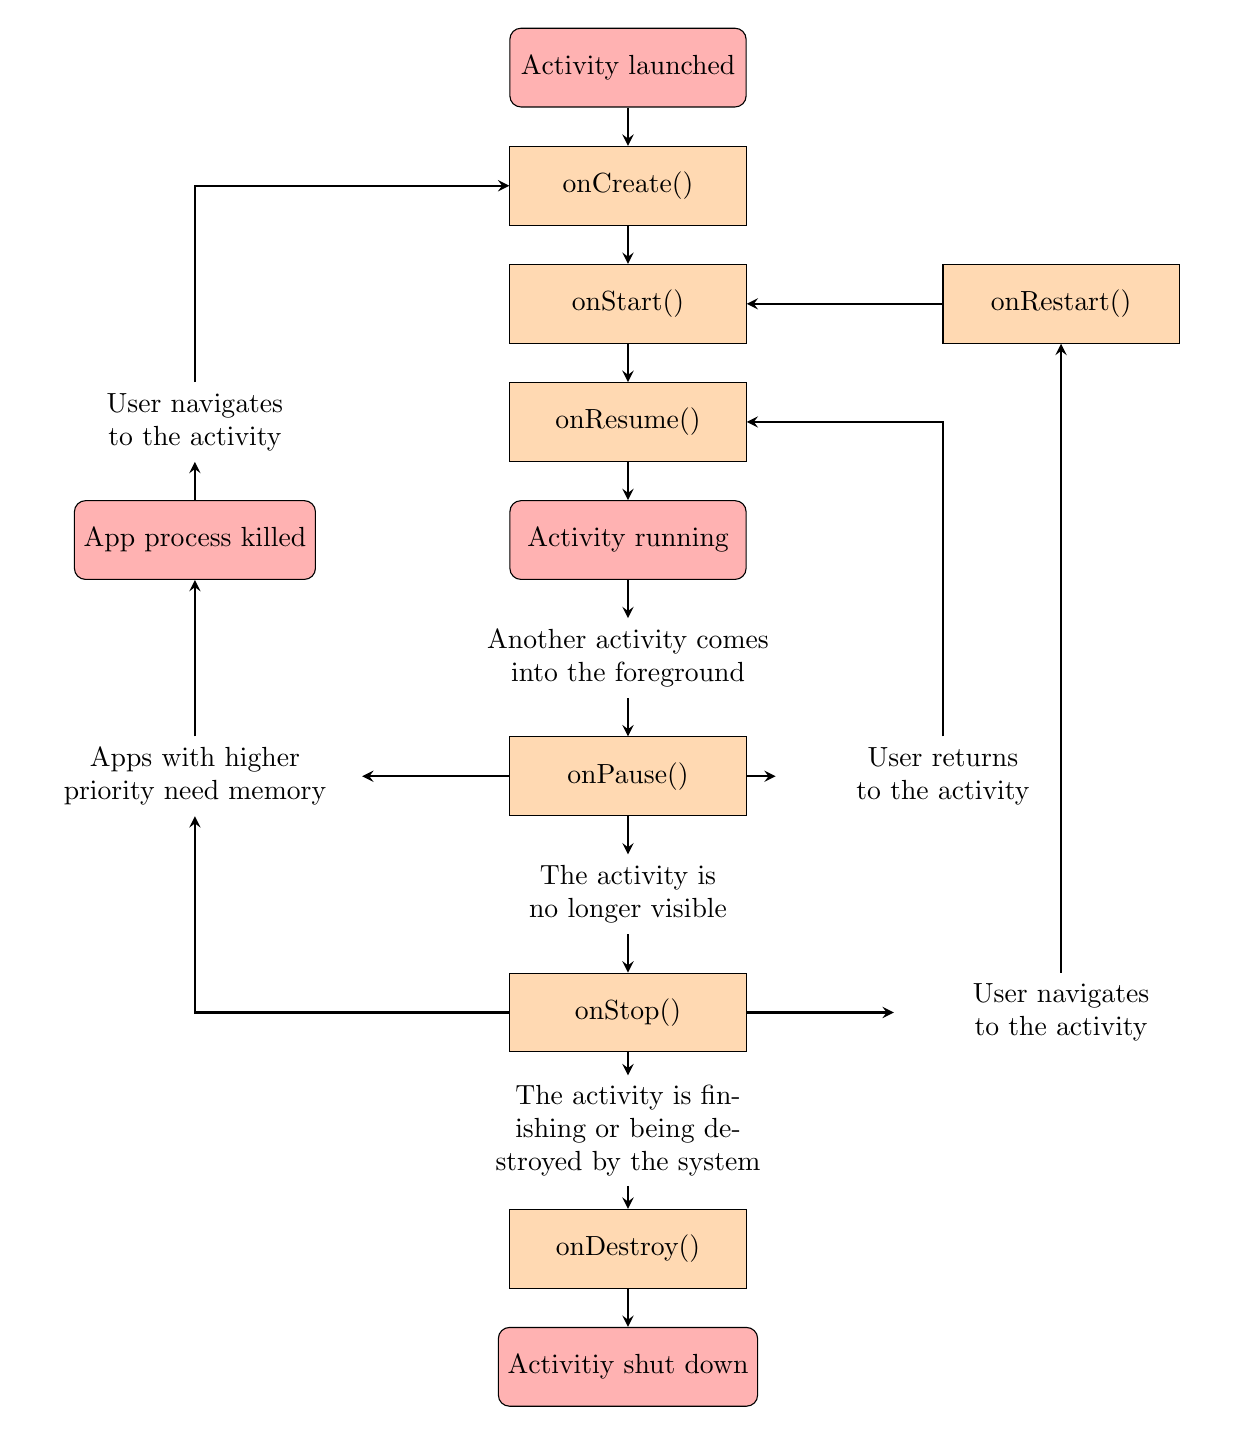
\begin{tikzpicture}[node distance=1.5cm]
			\node (start) [startstop] {Activity launched};
			\node (onCreate) [process, below of=start] {onCreate()};
			\node (onStart) [process, below of=onCreate] {onStart()};
			\node (onResume) [process, below of=onStart] {onResume()};
			\node (running) [startstop, below of=onResume] {Activity running};
			\node (commentOnPause) [comment, below of= running] {Another activity comes into the foreground};
			\node (onPause) [process, below of=commentOnPause] {onPause()};
			\node (commentOnStop) [comment, below of= onPause] {The activity is no longer visible};
			\node (onStop) [process, below of=commentOnStop] {onStop()};
			\node (commentOnDestroy) [comment, below of= onStop] {The activity is finishing or being destroyed by the system};
			\node (onDestroy) [process, below of=commentOnDestroy] {onDestroy()};
			\node (end) [startstop, below of=onDestroy] {Activitiy shut down};
			\node (onRestart) [process, right of=onStart, xshift=4cm] {onRestart()};
			\node (commentOnRestart) [comment, right of= onStop, xshift=4cm] {User navigates to the activity};
			\node (commentOnPauseRight) [comment, right of= onPause, xshift=2.5cm] {User returns to the activity};
			\node (commentOnPauseLeft) [comment, left of= onPause, xshift=-4cm] {Apps with higher priority need memory};
			\node (commentOnResumeLeft) [comment, left of= onResume, xshift=-4cm] {User navigates to the activity};
			\node (killed) [startstop, left of = running, xshift=-4cm] {App process killed};
			
			\draw [arrow] (start) -- (onCreate);
			\draw [arrow] (onCreate) -- (onStart);
			\draw [arrow] (onStart) -- (onResume);
			\draw [arrow] (onResume) -- (running);
			\draw [arrow] (running) -- (commentOnPause);
			\draw [arrow] (commentOnPause)  -- (onPause);
			\draw [arrow] (onPause) -- (commentOnStop);
			\draw [arrow] (commentOnStop) -- (onStop);
			\draw [arrow] (onStop) -- (commentOnDestroy);
			\draw [arrow] (commentOnDestroy) -- (onDestroy);
			\draw [arrow] (onDestroy) -- (end);
			\draw [arrow] (onRestart) -- (onStart);
			\draw [arrow] (onStop) -- (commentOnRestart);
			\draw [arrow] (commentOnRestart) -- (onRestart);
			\draw [arrow] (onPause) -- (commentOnPauseRight);
			\draw [arrow] (commentOnPauseRight) |- (onResume);
			\draw [arrow] (onPause) -> (commentOnPauseLeft);
			\draw [arrow] (onStop) -| (commentOnPauseLeft);
			\draw [arrow] (commentOnPauseLeft) -> (killed);
			\draw [arrow] (killed) -> (commentOnResumeLeft);
			\draw [arrow]  (commentOnResumeLeft) |- (onCreate);
			
		\end{tikzpicture}

\end{figure}

In figure \ref{fig:activity_life_cycle} one can see how various functions of the activity class are called depending in which state is the activity in following interaction with the user or with the Android operating system. The programmer has the possibilty to override these functions in order to customize the behaviour of the application.

In the following I will exemplify some of the methods as they are implemented in the Planes App. 

\begin{lstlisting} [caption = {onStop() life-cycle method},label=onStop_Android]
	override fun onStop() {
		m_SinglePlayerPreferencesService.writePreferences()
		m_MultiplayerPreferencesService.writePreferences()
		m_MainPreferencesService.writePreferences()
		m_VideoSettingsService.writePreferences()
		m_PlayersListService.stopPolling()
		m_ReceiveChatMessagesService.stopPolling()
		updateDatabaseFromNewMessagesFlags()
		super.onStop()
		Log.d("Planes", "onStop")
	}
\end{lstlisting}

In the onStop() method different screen configurations are saved in the so-called preferences of the app through calls of the method writePreferences(). The polling for the list of active players is stopped as well. The ROOM database is also updated with the information about the new messages.

\begin{lstlisting} [caption = {onResume() life-cycle method},label=onResume_Android]
	public override fun onResume() {
		super.onResume()
		if (m_MainPreferencesService.multiplayerVersion && m_MultiplayerRound.isUserLoggedIn()) {
			m_PlayersListService.startPolling()
			m_ReceiveChatMessagesService.startPolling()
			m_ReceiveChatMessagesService.setMainActivityUpdateFunction { updateNewMessagesFlags() }
		}
	}
\end{lstlisting}

In the onResume() method several configurations are made only for the the case when the user plays the multiplayer version and it is loogged in. These are:

\begin{itemize}
	\item Start polling for players' status
	\item Start polling for chat messages
	\item Configure the update of the main screen when receiving chat messages
	\item Update new messages flags on the top bar of the app
\end{itemize}


\subsubsection { Fragment }

Fragments represent a reusable portion of the UI. They are defined by their own layout files and have their own life cycle. They are hosted inside another fragment or an activity.

\subsubsection { Fragment Life Cycle }

\begin{figure}
	\caption{Fragment Life Cycle diagram as it is presented on the Android developer pages}
	\label{fig:fragment_life_cycle}
	\centering
	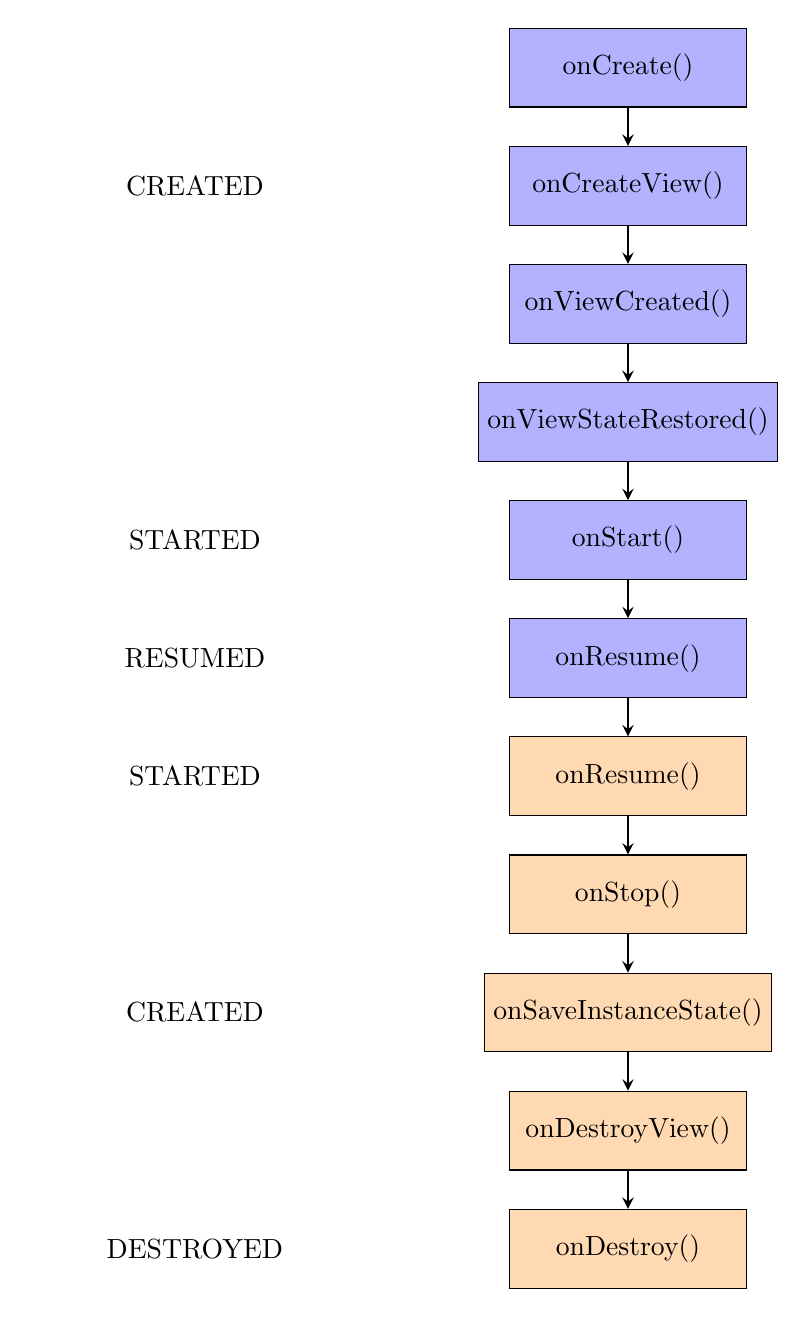
\begin{tikzpicture}[node distance=1.5cm]
		\node (onCreate) [processb] {onCreate()};
		\node (onCreateView) [processb, below of=onCreate] {onCreateView()};
		\node (onViewCreated) [processb, below of=onCreateView] {onViewCreated()};
		\node (onViewStateRestored) [processb, below of=onViewCreated] {onViewStateRestored()};
		\node (onStart) [processb, below of=onViewStateRestored] {onStart()};
		\node (onResume) [processb, below of= onStart] { onResume() };
		\node (onPause) [process, below of=onResume] {onResume()};
		\node (onStop) [process, below of= onPause] {onStop()};
		\node (onSaveInstanceState) [process, below of=onStop] {onSaveInstanceState()};
		\node (onDestroyView) [process, below of= onSaveInstanceState] {onDestroyView()};
		\node (onDestroy) [process, below of=onDestroyView] {onDestroy()};
		
		\node (ccreated) [comment, left of = onCreateView, xshift = -4cm] {CREATED};
		\node (cstarted) [comment, left of = onStart, xshift = -4cm] {STARTED};
		\node (cresumed) [comment, left of = onResume, xshift = -4cm] {RESUMED};
		\node (cstarted1) [comment, left of = onPause, xshift = -4cm] {STARTED};
		\node (ccreated1) [comment, left of = onSaveInstanceState, xshift = -4cm] {CREATED};
		\node (cdestroyed) [comment, left of = onDestroy, xshift = -4cm] {DESTROYED};
		
		\draw [arrow] (onCreate) -- (onCreateView);
		\draw [arrow] (onCreateView) -- (onViewCreated);
		\draw [arrow] (onViewCreated) -- (onViewStateRestored);
		\draw [arrow] (onViewStateRestored) -- (onStart);
		\draw [arrow] (onStart) -- (onResume);
		\draw [arrow] (onResume) -- (onPause);
		\draw [arrow] (onPause) -- (onStop);
		\draw [arrow] (onStop) -- (onSaveInstanceState);
		\draw [arrow] (onSaveInstanceState) -- (onDestroyView);
		\draw [arrow] (onDestroyView) -- (onDestroy);
	
	\end{tikzpicture}
	
\end{figure}

I am listing below a few life cycle methods from the CreateGameFragment which corresponds to the screen where the user connects to the game.

\begin{lstlisting}
	override fun onDetach () {
		super.onDetach()
		hideLoading()
		if (this::m_RefreshGameStatusSubscription.isInitialized)
		m_RefreshGameStatusSubscription.dispose()
		if (this::m_CreateGameSubscription.isInitialized)
		m_CreateGameSubscription.dispose()
		if (this::m_ConnectToGameSubscription.isInitialized)
		m_ConnectToGameSubscription.dispose()
		if (this::m_PollForOpponentSubscription.isInitialized)
		m_PollForOpponentSubscription.dispose()
	}
\end{lstlisting}

In the method onDetach() corresponding to the fragment being removed from the containing fragment or activity I am disposing network call objects. I am also hiding the loader animation corresponding to the user waiting for the opponent to connect to the game. 

\begin{lstlisting}
	 override fun onResume() {
		super.onResume()
		reinitializeFromState()
	}
\end{lstlisting}

\begin{lstlisting}
	private fun reinitializeFromState() {
		when(m_CreateGameSettingsService.createGameState) {
			CreateGameStates.NotSubmitted -> {
				binding.ProgressBarCreateGame.isVisible = false
				binding.startPlaying.isEnabled = false
			}
			CreateGameStates.Submitted -> {
				binding.ProgressBarCreateGame.isVisible = false
				binding.startPlaying.isEnabled = false
				checkGameStatus()
			}
			CreateGameStates.GameCreated -> { pollForGameConnection() }
			CreateGameStates.ConnectedToGame -> { connectedToGame() }
		}
	}
\end{lstlisting}

In the onResume() method the method reinitializeFromState() is called. This resets the screen to the state it had before being destroyed.

\subsection{Custom Views}

Most of the elements that appear in the XML Layout are derived from the class View, the basis of the hierarchy of displayable elements. In some cases it is required to create custom views. I will give now one from the PlanesAndroid application.

In order to achieve this mostly it is required to override the methods onDraw() and onMeasure().

\begin{lstlisting}
	public override fun onDraw(canvas: Canvas) {
		m_Paint.color = m_BackgroundColor
		canvas.drawRect(0f, 0f, width.toFloat(), height.toFloat(), m_Paint)
		m_Paint.color = m_ForegroundColor
		drawTextFitToSizeOneLine(m_Text, m_TextSize, canvas, m_Paint, width, height)
	}
\end{lstlisting}

The onDraw() method has a Canvas parameter which allows drawing onto. In this case a Rect is drawn with the specified background color along with a text with the specified foreground color. 

\begin{lstlisting}
	 override fun onMeasure(widthMeasureSpec: Int, heightMeasureSpec: Int) {
		val lp = layoutParams as PlanesVerticalLayoutParams
		if (!this::m_Text.isInitialized) m_Text = lp.getText()
		m_BackgroundColor = lp.getBackgroundColor().defaultColor
		m_ForegroundColor = lp.getForegroundColor().defaultColor
		val measuredHeight = measureHeightOneLineText(heightMeasureSpec, m_Paint, m_Text)
		val measuredWidth = measureWidthOneLineText(widthMeasureSpec, m_Paint, m_Text)
		setMeasuredDimension(measuredWidth, measuredHeight)
	}
\end{lstlisting}

In the onMeasure() method the layout parameters of the view are being read: the background color, the foreground color and the text to be displayed.

\begin{lstlisting}
	fun measureHeightOneLineText(measureSpec: Int, paint: Paint, text: String): Int {
		View.MeasureSpec.getMode(measureSpec)
		val specSize = View.MeasureSpec.getSize(measureSpec)
		var resultHeight = 10
		paint.textSize = 20f
		val bounds = Rect()
		paint.getTextBounds(text, 0, text.length, bounds)
		if (bounds.height() > resultHeight) resultHeight = bounds.height()
		if (specSize > resultHeight) resultHeight = specSize
		return resultHeight
	}
\end{lstlisting}

The height of the View is being calculated in the function measureHeightOneLineText() as follows: first the size of the text is being determined from the paint object, if it is bigger than the minimum dimension of 10 than this is considered as the intermediary height of the View, further more if the specificated height is still bigger than this intermediary value, the specified height is taken as the View's height.

A similar reasoning is used for determining the View's width. Finally with the help of the function setMeasuredDimension() the calculated dimensions of the View are set.

\subsection {Custom Layouts}



\section{PlanesCompose}

Following new developments of Android development libraries I am porting the project to a new technology: JetPack Compose. 

\subsection{Navigation}

The basis of the application is the navigation. Here I wish to keep the drawer navigation. 
The navigation drawer and main screen content are defined as follows (\ref{drawer_compose})

\begin{lstlisting}  [caption = {Drawer Navigation in Jetpack Compose},label=drawer_compose]
	ModalNavigationDrawer(
	drawerState = drawerState,
	drawerContent = {
		ModalDrawerSheet {
			DrawerContent(navController = navController,
			drawerScope = scope,
			drawerState = drawerState)
		}
	},
	gesturesEnabled = true
	) {
		Scaffold(
		topBar = {
			TopBar(
			modifier = Modifier.padding(30.dp)
			.height(100.dp).fillMaxWidth(),
			onOpenDrawer = {
				scope.launch {
					drawerState.apply {
						if (isClosed)
						open()
						else
						close()
					}
				}
			},
			currentScreenName = currentScreenState.value
			)
		}
		) { padding ->
			ScreenContent(modifier = Modifier.padding(padding),
			currentScreenState = currentScreenState,
			navController = navController)
		}
	}
\end{lstlisting}

The design of the drawer is defined under the drawer\_content variable. The layout of the application screen is defined under the ending lambda of the ModalNavigationDrawer composable . 

In listing \ref{drawer_layout__compose} the structure of the drawer is shown. Probably this is not the final code for the drawer but the principle will stay the same. So the drawer is a Column layout in which screen names are stacked one under another. The screen names are grouped in sections and a HorizontalDivider is shown between sections .

\begin{lstlisting} [caption = {Drawer View},label=drawer_layout__compose]
	@Composable
	fun DrawerContent(modifier: Modifier = Modifier,
	navController: NavController,
	drawerScope: CoroutineScope,
	drawerState: DrawerState,
	) {
		
		Column(
		modifier = Modifier.padding(horizontal = 16.dp)
		.verticalScroll(rememberScrollState())
		) {
			Text(
			text = "Planes",
			modifier = Modifier.padding(16.dp),
			style = MaterialTheme.typography.titleLarge
			)
			
			HorizontalDivider()
			
			DrawerMenuItemGeneric("Login", {
				drawerScope.launch {
					drawerState.close()
				}
				navController.navigate(route = PlanesScreens.Login.name)
			})
			
			DrawerMenuItemGeneric("Logout", {
				drawerScope.launch {
					drawerState.close()
				}
				navController.navigate(route = PlanesScreens.Logout.name)
			})
			
			DrawerMenuItemGeneric("Register", {
				drawerScope.launch {
					drawerState.close()
				}
				navController.navigate(route = PlanesScreens.Register.name)
			})
			
			DrawerMenuItemGeneric("Chat", {
				drawerScope.launch {
					drawerState.close()
				}
				navController.navigate(route = PlanesScreens.Chat.name)
			})
			
			Text(
			text = "Single Player Game",
			modifier = Modifier.padding(16.dp),
			style = MaterialTheme.typography.titleMedium
			)
			DrawerMenuItemGeneric("Game", {
				drawerScope.launch {
					drawerState.close()
				}
				navController.navigate(route = PlanesScreens.SinglePlayerGame.name)
			})
			
			DrawerMenuItemGeneric("Preferences", {
				drawerScope.launch {
					drawerState.close()
				}
				navController.navigate(route = PlanesScreens.SinglePlayerPreferences.name)
			})
			
			DrawerMenuItemGeneric("Game Statistics", {
				drawerScope.launch {
					drawerState.close()
				}
				navController.navigate(route = PlanesScreens.SinglePlayerGameStatistics.name)
			})
			
			
			Text(
			text = "Multiplayer Game",
			modifier = Modifier.padding(16.dp),
			style = MaterialTheme.typography.titleMedium
			)
			DrawerMenuItemGeneric("Game", {
				drawerScope.launch {
					drawerState.close()
				}
				navController.navigate(route = PlanesScreens.MultiplayerGame.name)
			})
			
			DrawerMenuItemGeneric("Preferences", {
				drawerScope.launch {
					drawerState.close()
				}
				navController.navigate(route = PlanesScreens.MultiplayerPreferences.name)
			})
			
			DrawerMenuItemGeneric("Game Statistics", {
				drawerScope.launch {
					drawerState.close()
				}
				navController.navigate(route = PlanesScreens.MultiplayerGameStatistics.name)
			})
			
			Text(
			text = "Info",
			modifier = Modifier.padding(16.dp),
			style = MaterialTheme.typography.titleMedium
			)
			
			DrawerMenuItemGeneric("About", {
				drawerScope.launch {
					drawerState.close()
				}
				navController.navigate(route = PlanesScreens.Info.name)
			})
			
			DrawerMenuItemGeneric("Tutorials", {
				drawerScope.launch {
					drawerState.close()
				}
				navController.navigate(route = PlanesScreens.Tutorials.name)
			})
			
			DrawerMenuItemGeneric("Delete User", {
				drawerScope.launch {
					drawerState.close()
				}
				navController.navigate(route = PlanesScreens.DeleteUser.name)
			})
		}
	}
\end{lstlisting}

Each screen name is represented by an element of the composable DrawerMenuItemGeneric which receive parameters the screen name and a lambda function that it is to be called when the screen name is clicked. The call navController.navigate() makes the screen transition. It corresponds to the supportFragmentManager.beginTransaction() from \ref{start_norobot_fragment}.

\subsection{Main Screen}

The structure of the application screen is also defined in listing \ref{drawer_compose} which is the definition of the drawer navigation. This is defined with a Scaffold composable composed of a top bar together with the content of the screen.

\begin{lstlisting} [caption = {Main Screen Layout},label=main_screen]
	Scaffold(
	topBar = {
		TopBar(
		modifier = Modifier.padding(30.dp)
		.height(100.dp).fillMaxWidth(),
		onOpenDrawer = {
			scope.launch {
				drawerState.apply {
					if (isClosed)
					open()
					else
					close()
				}
			}
		},
		currentScreenName = currentScreenState.value
		)
	}
	) { padding ->
		ScreenContent(modifier = Modifier.padding(padding),
		currentScreenState = currentScreenState,
		navController = navController)
	}
\end{lstlisting} 

TopBar is defined as follows:

\begin{lstlisting}  [caption = {Top Bar},label=top_bar]
	TopBar(modifier: Modifier = Modifier,
	onOpenDrawer: () -> Unit = {},
	currentScreenName: String
	) {
		TopAppBar(
		colors = TopAppBarDefaults.topAppBarColors(
		containerColor = MaterialTheme.colorScheme.surfaceVariant
		),
		navigationIcon = {
			Icon(
			imageVector = Icons.Default.Menu,
			contentDescription = "Navigation Icon",
			modifier = Modifier.clickable {
				onOpenDrawer()
			}. padding(start = 16.dp, end = 8.dp)
			.size(28.dp))
		},
		title = {
			Text(text = currentScreenName)
		},
		actions = {
			Icon(
			imageVector = Icons.Default.AccountBox,
			contentDescription = "Navigation Icon",
			modifier = Modifier.padding(start = 16.dp, end = 8.dp).size(28.dp)
			)
			Icon(
			imageVector = Icons.Default.Notifications,
			contentDescription = "Navigation Icon",
			modifier = Modifier.padding(start = 16.dp, end = 8.dp)
			.size(28.dp))
		}
		)
	}
	
\end{lstlisting}

This uses the predefined composable TopAppBar which receives as parameters a navigation icon (the Hamburger button), the title displayed as well as actions which can be added to this bar to be called from everywhere in the app. The variable currentScreenName is defined such that when a new screen is shown the title of the screen is displayed in the top bar.

The ScreenContent composable defines the changing content of the main screen as follows:

\begin{lstlisting}
	@Composable
	fun ScreenContent(modifier: Modifier, currentScreenState: MutableState<String>,
	navController: NavHostController
	) {
		PlanesNavigation(modifier = modifier,
		currentScreenState, navController,
		context = LocalContext.current)
	}
\end{lstlisting}

PlanesNavigation is a composable that associates to the application screen names composable functions representing the respective screens.

\begin{lstlisting}
	@Composable
	fun PlanesNavigation(modifier: Modifier, currentScreenState: MutableState<String>,
	navController: NavHostController, context: Context) {
		
		NavHost(
		navController = navController,
		startDestination = PlanesScreens.Info.name) {
			composable(PlanesScreens.SinglePlayerGame.name) {
				SinglePlayerGameScreen(modifier = modifier, currentScreenState, navController = navController)
			}
			composable(PlanesScreens.SinglePlayerGameStatistics.name) {
				SinglePlayerGameStatisticsScreen(modifier = modifier, currentScreenState, navController = navController)
			}
			composable(PlanesScreens.SinglePlayerPreferences.name) {
				SinglePlayerPreferencesScreen(modifier = modifier, currentScreenState, navController = navController)
			}
			composable(PlanesScreens.MultiplayerGame.name) {
				MultiplayerGameScreen(modifier = modifier, currentScreenState, navController = navController)
			}
			composable(PlanesScreens.MultiplayerGameStatistics.name) {
				MultiplayerGameStatisticsScreen(modifier = modifier, currentScreenState, navController = navController)
			}
			composable(PlanesScreens.MultiplayerPreferences.name) {
				MultiplayerPreferencesScreen(modifier = modifier, currentScreenState, navController = navController)
			}
			composable(PlanesScreens.Info.name) {
				AboutScreen(modifier = modifier, currentScreenState, navController = navController,
				aboutEntryList = AboutEntryRepository.create("0.1", context = context))
			}
			composable(PlanesScreens.Tutorials.name) {
				VideoScreen(modifier = modifier, currentScreenState, navController = navController)
			}
			composable(PlanesScreens.Login.name) {
				LoginScreen(modifier = modifier, currentScreenState, navController = navController)
			}
			composable(PlanesScreens.Logout.name) {
				LogoutScreen(modifier = modifier, currentScreenState, navController = navController)
			}
			composable(PlanesScreens.Register.name) {
				RegisterScreen(modifier = modifier, currentScreenState, navController = navController)
			}
			composable(PlanesScreens.DeleteUser.name) {
				DeleteUserScreen(modifier = modifier, currentScreenState, navController = navController)
			}
			composable(PlanesScreens.Chat.name) {
				ChatScreen(modifier = modifier, currentScreenState, navController = navController)
			}
		}
\end{lstlisting}

\subsection{Info Screen}

In this version of the Planes App the contents of the info screen is the same as in the PlanesAndroid app. But the JetPackCompose framework does not offer a Recycler View anymore. Let's see how the functionality is replicated in this case.

A data model class is used which is identical to the one used for the Recycler View. I only gave it a different name: AboutEntryModel. The method for creating the data repository is the same, it is only integrated in the companion object of a class called AboutEntryRepository. 

The layout for one entry in the About Screen is now created with a composable function.

\begin{lstlisting}
	fun AboutEntryRow(entry: AboutEntryModel, context: Context) {
		
		val uriHandler = LocalUriHandler.current
		
		Column(modifier = Modifier.padding(4.dp).
		fillMaxWidth())
		{
			Text(text = entry.getTitle(),
			style = MaterialTheme.typography.titleMedium)
			Text(text = entry.getText(),
			style = MaterialTheme.typography.bodyMedium)
			if (entry.hasButton()) {
				Button(modifier = Modifier.align(Alignment.End),
				onClick = {
					uriHandler.openUri(entry.getLinkButton())
				}) {
					Text(text = entry.getTextButton())
				}
			}
		}
	}
\end{lstlisting}

The difference from \ref{layout_button_info_screen} and \ref{layout_with_button_info_screen} is that a single construct is needed to create the layout. This is possible through the if command in the AboutEntryRow composable.

Finally to glue everything together a LazyColumn composable is used as follows:

\begin{lstlisting}
	fun AboutScreen(modifier: Modifier, currentScreenState: MutableState<String>,
	context: Context, navController: NavController,
	aboutEntryList: List<AboutEntryModel>) {
		
		currentScreenState.value = PlanesScreens.Info.name
		
		Surface(modifier = modifier,
		color = MaterialTheme.colorScheme.background) {
			Column(modifier = Modifier.fillMaxWidth(),
			horizontalAlignment = Alignment.CenterHorizontally,
			verticalArrangement = Arrangement.Center) {
				LazyColumn {
					items(items = aboutEntryList) {
						AboutEntryRow(entry = it, context)
					}
				}
			}
		}
	}
\end{lstlisting}

I personally prefer the implementation in JetPackCompose as it is simpler and eleganter.

\subsection {Video Screen}

For the video screen I am using the Exoplayer library. The definition of the player is as follows:

\begin{lstlisting}
	fun VideoPlayer(videoId : Int) {
		val context = LocalContext.current
		
		val exoPlayer = remember(context) {
			ExoPlayer.Builder(context).build().apply {
				val dataSourceFactory: DataSource.Factory = DefaultDataSource.Factory(context, DefaultHttpDataSource.Factory())
				val uriSource = Uri.parse(
				"android.resource://"
				+ context.packageName + "/" + videoId)
				val source = ProgressiveMediaSource.Factory(dataSourceFactory)
				.createMediaSource(
				MediaItem.fromUri(uriSource))
				this.setMediaSource(source)
				this.prepare()
			}
		}
		
		
		AndroidView(
		factory = { ctxt ->
			PlayerView(ctxt).apply {
				player = exoPlayer
				layoutParams = ViewGroup.LayoutParams(
				ViewGroup.LayoutParams.MATCH_PARENT,
				ViewGroup.LayoutParams.WRAP_CONTENT
				)
			}
		},
		update = { pview ->
			pview.apply {
				val player = this.player!!
				val uriSource = Uri.parse(
				"android.resource://"
				+ context.packageName + "/" + videoId)
				player.setMediaItem(MediaItem.fromUri(uriSource))
				player.prepare()
				//player.playWhenReady = true
				
			}
		},
		onReset = { pview ->
			pview.player = null
		}
		)
\end{lstlisting}

The composable function receives as parameter the videoId and initializes the player with the video defined by this id. 

To define the layout of the video buttons which allow navigating to different tutorial videos I am using at first a helper function which defines the VideoButton.

\begin{lstlisting}
	fun VideoButton(entry: VideoModel, currentVideoState: MutableState<Int>, modifier: Modifier) {
		Card(
		modifier.padding(1.dp).clickable {
			currentVideoState.value = entry.getVideoId()
		}.wrapContentHeight(),
		shape = RectangleShape,
		colors = CardDefaults.cardColors(
		containerColor = MaterialTheme.colorScheme.surfaceVariant
		)
		) {
			Column(
			verticalArrangement = Arrangement.Center,
			horizontalAlignment = Alignment.CenterHorizontally,
			modifier = Modifier.fillMaxSize()
			) {
				Text(
				modifier = Modifier.align(Alignment.CenterHorizontally),
				text = entry.getVideoName()
				)
			}
		}
	}
\end{lstlisting}

Then the layout of these buttons is defined with the composable LazyVerticalGrid, for portrait orientation, and with the composable LazyColumn, for landscape orientation.

\begin{lstlisting}
fun VideoScreen(modifier: Modifier, currentScreenState: MutableState<String>,
navController: NavController, videoModelList: List<VideoModel>) {
	
	currentScreenState.value = PlanesScreens.Tutorials.name
	val configuration = LocalConfiguration.current
	val currentVideoState = remember {
		mutableStateOf(R.raw.guessing)
	}
	
	Column(
	modifier = modifier,
	verticalArrangement = Arrangement.Center,
	horizontalAlignment = Alignment.CenterHorizontally
	) {
	when (configuration.orientation) {
		Configuration.ORIENTATION_PORTRAIT -> {
			
		Column(verticalArrangement = Arrangement.spacedBy(1.dp)) {
			VideoPlayer(currentVideoState.value)
			LazyVerticalGrid(
			columns = GridCells.Fixed(2),
			verticalArrangement = Arrangement.spacedBy(1.dp),
			horizontalArrangement = Arrangement.spacedBy(1.dp),
			contentPadding = PaddingValues(1.dp)
			) {
				items(items = videoModelList) { entry ->
					VideoButton(entry, currentVideoState, Modifier.width(200.dp).height(100.dp))
				}
			}
		}
		}
		else -> {
			Row() {
			Column(verticalArrangement = Arrangement.spacedBy(1.dp)) {
				Spacer(modifier = Modifier)
				LazyColumn(
				verticalArrangement = Arrangement.spacedBy(1.dp),
				contentPadding = PaddingValues(
				top = 1.dp,
				bottom = 1.dp
				)
				) {
					items(items = videoModelList) { entry ->
						VideoButton(entry, currentVideoState, Modifier.width(200.dp).height(100.dp))
					}
				}
			}
			
			VideoPlayer(currentVideoState.value)
			}
		}
	}
}
}
\end{lstlisting}

\subsection{Preferences Screen}

The preferences screen is defined as a composable function which takes a view model (optionsViewModel) as parameter:

\begin{lstlisting}
	
	fun PreferencesScreen(modifier: Modifier,
	currentScreenState: MutableState<String>,
	navController: NavController,
	optionsViewModel: PreferencesViewModel
	) {
		
		
		currentScreenState.value = PlanesScreens.Preferences.name
		val scrollState = rememberScrollState()
		
		val keyboardController = LocalSoftwareKeyboardController.current
		
		Column(modifier = modifier.fillMaxSize().padding(start = 15.dp).
		verticalScroll(state = scrollState),
		verticalArrangement = Arrangement.Top,
		horizontalAlignment = Alignment.Start) {
			
			val computerSkillsArray = stringArrayResource(R.array.computer_skills)
			
			Column(modifier = Modifier.padding(start = 15.dp, top = 10.dp))  {
				
				Text(text = stringResource(R.string.computer_skill),
				modifier = Modifier.padding(start = 15.dp))
				
				CheckBoxOption(text = computerSkillsArray[0],
				optionsViewModel.getComputerSkill() == 0,
				{optionsViewModel.setComputerSkill(0)})
				CheckBoxOption(text = computerSkillsArray[1],
				optionsViewModel.getComputerSkill() == 1,
				{optionsViewModel.setComputerSkill(1)})
				CheckBoxOption(text = computerSkillsArray[2],
				optionsViewModel.getComputerSkill() == 2,
				{optionsViewModel.setComputerSkill(2)})
				
			}
			
			
			val yesNoOptionsArray = stringArrayResource(R.array.yesno_options)
			Column(modifier = Modifier.padding(start = 15.dp, top = 10.dp)) {
				
				Text(text = stringResource(R.string.show_plane_after_kill),
				modifier = Modifier.padding(start = 15.dp))
				
				CheckBoxOption(text = yesNoOptionsArray[0],
				optionsViewModel.getShowPlaneAfterKill(),
				{optionsViewModel.setShowPlaneAfterKill(true)})
				CheckBoxOption(text = yesNoOptionsArray[1],
				!optionsViewModel.getShowPlaneAfterKill(),
				{optionsViewModel.setShowPlaneAfterKill(false)})
				
			}
			
			
			CommonTextField(modifier = Modifier.padding(15.dp),
			optionsViewModel,
			{ prefs ->  prefs.getUserName()},
			{ prefs, str -> prefs.setUserName(str)},
			onAction = KeyboardActions {
				keyboardController?.hide()
			},
			keyboardType = KeyboardType.Text,
			imeAction = ImeAction.Default,
			placeholder = stringResource(R.string.username))
			
			
			
			CommonTextField(
			modifier = Modifier.padding(15.dp),
			optionsViewModel,
			{ prefs -> prefs.getPassword() },
			{ prefs, str -> prefs.setPassword(str) },
			onAction = KeyboardActions {
				keyboardController?.hide()
			},
			keyboardType = KeyboardType.Text,
			imeAction = ImeAction.Default,
			placeholder = stringResource(R.string.password)
			)
			
		}
\end{lstlisting}

The persistence of the preferences is implemented inside the view model class:

\begin{lstlisting}
class PreferencesViewModel @Inject constructor(
private val dataStore: DataStore<Preferences>
): ViewModel() {
	
	private companion object {
		val COMPUTER_SKILL = intPreferencesKey("computer_skill")
		val SHOW_PLANE = booleanPreferencesKey("show_plane")
		val USERNAME = stringPreferencesKey("username")
		val PASSWORD = stringPreferencesKey("password")
	}
	
	private var m_ComputerSkill = mutableStateOf(2)
	private var m_ShowPlaneAfterKill = mutableStateOf(false)
	private var m_UserName = mutableStateOf("")
	private var m_Password = mutableStateOf("")
	
	fun getComputerSkill(): Int {
		return m_ComputerSkill.value
	}
	
	fun setComputerSkill(value: Int) {
		m_ComputerSkill.value = value
		
		viewModelScope.launch {
			dataStore.edit { prefs ->
				prefs[COMPUTER_SKILL] = value
			}
		}
	}
	
	fun getShowPlaneAfterKill() : Boolean {
		return m_ShowPlaneAfterKill.value
	}
	
	fun setShowPlaneAfterKill(value: Boolean) {
		m_ShowPlaneAfterKill.value = value
		
		viewModelScope.launch {
			dataStore.edit { prefs ->
				prefs[SHOW_PLANE] = value
			}
		}
	}
	
	fun getUserName(): String {
		return m_UserName.value
	}
	
	fun setUserName(value: String) {
		m_UserName.value = value
		
		viewModelScope.launch {
			dataStore.edit { prefs ->
				prefs[USERNAME] = value
			}
		}
	}
	
	fun getPassword(): String {
		return m_Password.value
	}
	
	fun setPassword(value: String) {
		m_Password.value = value
		
		viewModelScope.launch {
			dataStore.edit { prefs ->
				prefs[PASSWORD] = value
			}
		}
	}
	
	
	init {
		updateFields()
	}
	
	private fun updateFields() {
		viewModelScope.launch {
			dataStore.data.map { prefs ->
				UserPreferences(
				computerSkill = prefs[COMPUTER_SKILL] ?: 2,
				showPlaneAfterKill = prefs[SHOW_PLANE] ?: false,
				userName = prefs[USERNAME] ?: "",
				password = prefs[PASSWORD] ?: "")
				
			}.collect { userprefs ->
				
				m_ComputerSkill.value = userprefs.computerSkill
				m_ShowPlaneAfterKill.value = userprefs.showPlaneAfterKill
				m_UserName.value = userprefs.userName
				m_Password.value = userprefs.password
			}
			
		}
	}
	
	fun savePreferences() {
		viewModelScope.launch {
			dataStore.edit { prefs ->
				prefs[COMPUTER_SKILL] = m_ComputerSkill.value
				prefs[SHOW_PLANE] = m_ShowPlaneAfterKill.value
				prefs[USERNAME] = m_UserName.value
				prefs[PASSWORD] = m_Password.value
			}
		}
	}
	
}
\end{lstlisting}

This view model is not a simple data class like the implementation in \ref{pref_view_model1}. It derives from ViewModel and it is injected into the composables with dependency injection. It keeps its state when screen orientation is changed for example. 

The view model is connected to the composable (PreferencesScreen) defining the preference screen where it is given as parameter (optionsViewModel). In order for it to work smoothly with input methods like typing of username and password, it keeps the preferences elements into MutableState variables. MutableState variables are state holding variables whose change can be tracked by JetPack Compose. When the value change occurs some composable functions will be recomputed to update the interface.

In addition to saving inputs into the MutableState variables, they are persisted into a Data Store that is meant to keep the settings beyond stopping of the app. The data store is a newer alternative to the shared preferences used in \ref{pres_prefs1}

This is implemented for example in this method:

\begin{lstlisting}
	fun setShowPlaneAfterKill(value: Boolean) {
		m_ShowPlaneAfterKill.value = value
		
		viewModelScope.launch {
			dataStore.edit { prefs ->
				prefs[SHOW_PLANE] = value
			}
		}
	}
\end{lstlisting}

m\_ShowPlaneAfterKill is a MutableState variable which keeps the user option during the functioning of the application. Every time the user changes these options, this change is persisted through a coroutine (a kind of lightweight background job) to the data store. When the preferences value are required in the Preferences Screen they are delivered directly from the MutableState variables.

When the view model is first instantiated the values from the data store are read into the MutableState variables:

\begin{lstlisting}
	private fun updateFields() {
		viewModelScope.launch {
			dataStore.data.map { prefs ->
				UserPreferences(
				computerSkill = prefs[COMPUTER_SKILL] ?: 2,
				showPlaneAfterKill = prefs[SHOW_PLANE] ?: false,
				userName = prefs[USERNAME] ?: "",
				password = prefs[PASSWORD] ?: "")
			}.collect { userprefs ->
				m_ComputerSkill.value = userprefs.computerSkill
				m_ShowPlaneAfterKill.value = userprefs.showPlaneAfterKill
				m_UserName.value = userprefs.userName
				m_Password.value = userprefs.password
			}	
		}
	}
\end{lstlisting}

\subsection { Android Concepts }

\subsubsection { Composable Functions }
\subsubsection { Coroutines }